%
%	Begrifflichkeiten
%

\pagebreak
\section{Data Source and Wrangling}

\onehalfspacing

\subsection{Data Source}

\subsubsection{The Group}

\subsubsection{The Blog}

\subsubsection{Social Media and Loneliness}

According to a recent study conducted by the American Psychological Association, social distancing over an extended period can increase loneliness and significantly affect people's health.\footnote{See \textit{Luchetti, M. (2020)}: The trajectory of loneliness in response to COVID-19. \cite{apaLoneliness}}

\subsubsection{Hate Speech}

\subsubsection{Ableism}

\subsubsection{Climate Anxiety}

\subsection{Web Traffic Analysis}

\subsubsection{Web Traffic KPIs}

\subsubsection{Data Collection}

\subsection{Data Wrangling}

\subsubsection{Original Columns}

We have six files in total. First, let's have a look at each of the files' contents and the original columns.

The wp-comments table holds all information pertaining to comments, which will greatly help us in evaluating engagement with the individual posts.
\begin{lstlisting}[caption=wp-comments, frame=single, basicstyle=\ttfamily]
"comment-ID", "comment-post-ID", "comment-author", 
"comment-author-email", "comment-author-url", 
"comment-author-IP", "comment-date", "comment-date-gmt", 
"comment-content", "comment-approved", "comment-parent", 
"comment-type", "user-id", "comment-alter-id", 
"meta:ct-checked", "meta:ct-checked-now", "meta:ct-bad", 
"meta:ct-hash", "meta:akismet-result", 
"meta:akismet-history", "meta:akismet-as-submitted"
\end{lstlisting}

\subsubsection{Removing PII}

There's quite a lot of personally identifiable information in these tables that I will remove before starting the analysis:

\begin{itemize}
 \item wp-admin: The information in this table is only affecting me as the author of the paper, so no change is necessary
 \item wp-comments: I'll remove anything that could potentially identify the person commenting as well as all meta information and an empty column.
 \item wp-pages: The table has no personally identifiable information
 \item wp-search: The table has no personally identifiable information
 \item wp-visit: The table has no personally identifiable information
 \item wp-visitor: I'll remove all information, including IP Address, that could potentially identify the visitor
\end{itemize}

Removing columns from CSV files is an easy task for any spreadsheet program.

\subsubsection{GDPR Compliance}

\subsubsection{Removing Spam}

To do this I use the shell and filter approximately 18000 page impressions:

\begin{lstlisting}[caption=Removing Spam, frame=single, basicstyle=\ttfamily]
$ wc -l wp-visitor-2021-04-05.csv
68027 wp-visitor-2021-04-05.csv

$ fgrep -e "DE" wp-visitor-2021-04-05.csv | wc -l
49883

$ fgrep -e "AT" wp-visitor-2021-04-05.csv | wc -l
519

$ fgrep -e "CH" wp-visitor-2021-04-05.csv | wc -l
264

$ fgrep -e "CH" -e "AT" -e "DE" wp-visitor-2021-04-05.csv \
  > wp-visitor-2021-04-05-nospam.csv

$ wc -l wp-visitor-2021-04-05-nospam.csv 
50564 wp-visitor-2021-04-05-nospam.csv
\end{lstlisting}

\subsubsection{Count Data Notebook}

\begin{figure}[H]
\centering
\caption {Database Tables}
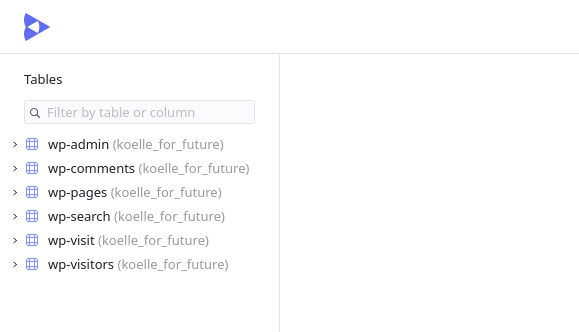
\includegraphics[width=\linewidth]{images/tables.png}
\label{fig:tablesCount}
\end{figure}

